\appendix

\chapter{TLS-Automatenmodelle}
\label{cha_tls_state_machines}

\begin{figure}[H]
	\centering
	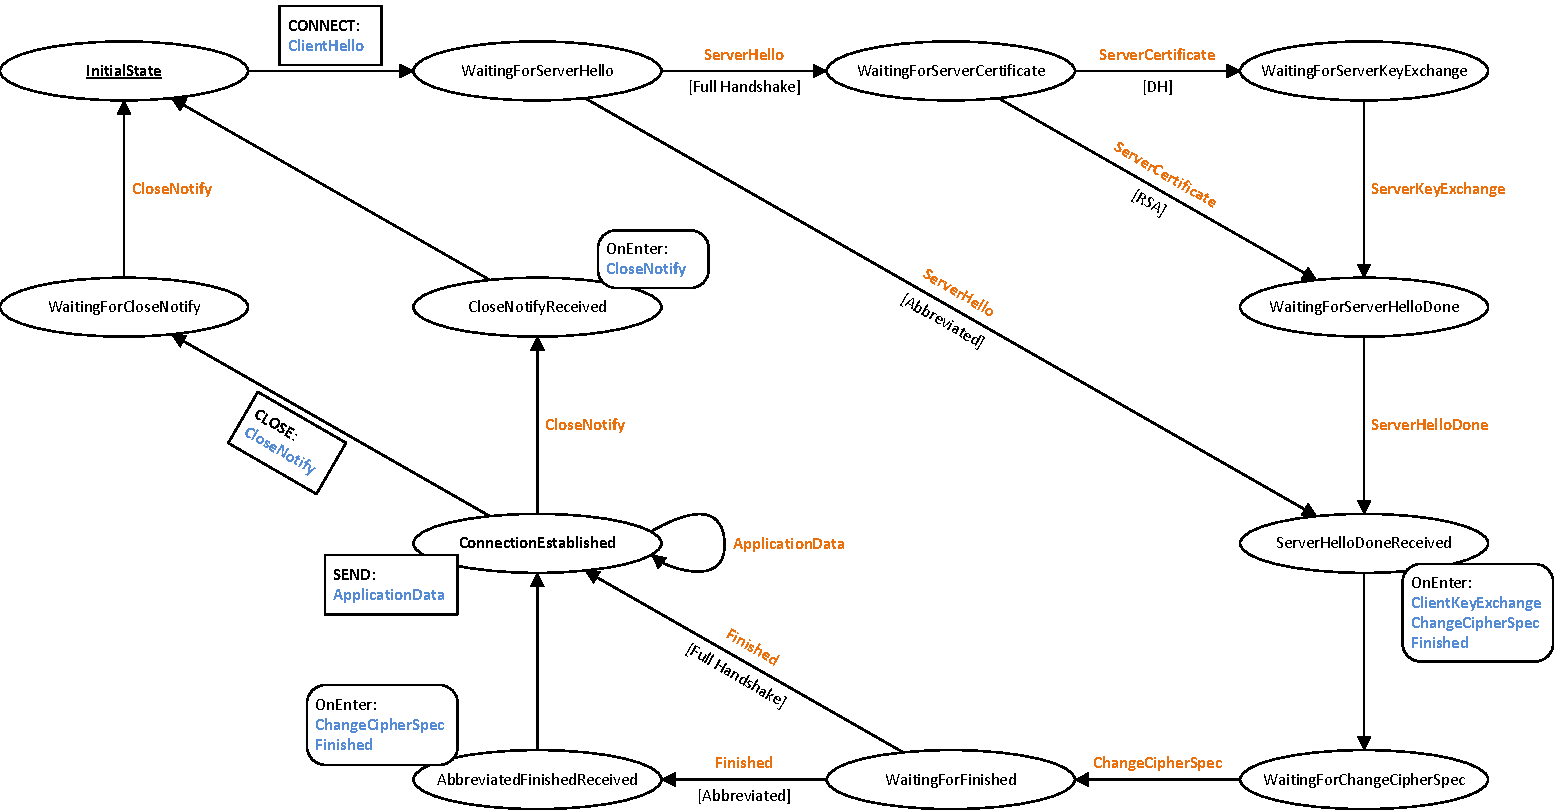
\includegraphics[scale=0.75, angle = 90]{Diagrams/statemachines/client_state_machine.pdf} %
	\caption{Das Automatenmodell für den TLS-Client}
	\label{fig_tls_client_state_machine}
\end{figure}

\begin{figure}[H]
	\centering
	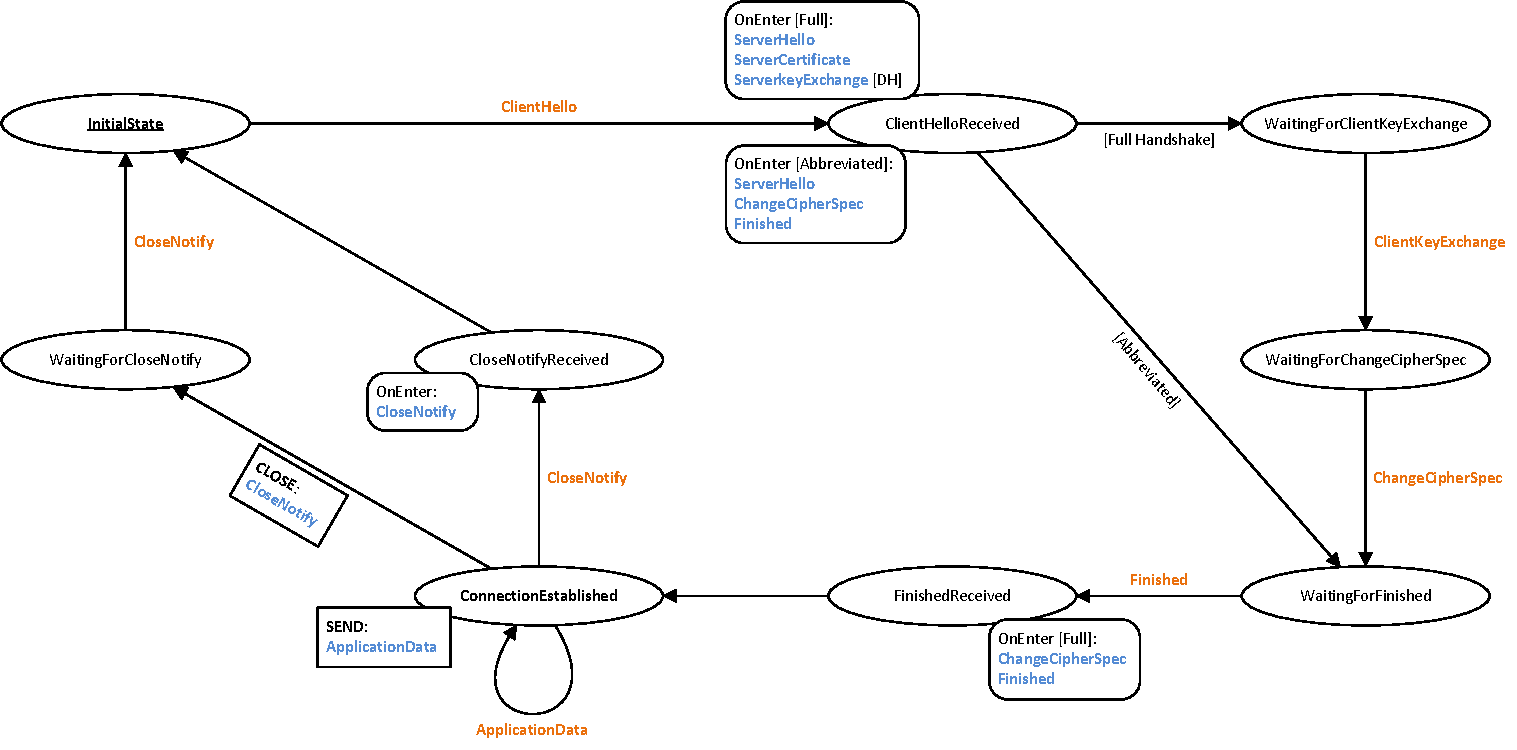
\includegraphics[scale=0.75, angle = 90]{Diagrams/statemachines/server_state_machine.pdf} %
	\caption{Das Automatenmodell für den TLS-Server}
	\label{fig_tls_server_state_machine}
\end{figure}


\chapter{Erweiterung der Anwendung}

In diesem Abschnitt soll anhand eines einfachen Beispiels gezeigt werden, was bei der Erweiterung der Anwendung um ein weiteres Protokoll zu beachten ist. Dazu wird ein einfaches Protokoll betrachtet, bei dem eine Nachricht lediglich aus einem Längenfeld und einem Nachrichteninhalt besteht. Ein Client kann Nachrichten dieses Formats an den Server senden, der diese lediglich genauso zurücksendet. Es handelt sich also um eine leicht modifizierte Variante des Echo-Protokolls\footnote{Das Echo-Protokoll wird in RFC 862 spezifiziert.}.

Im ersten Schritt wird der Nachrichtentyp implementiert (siehe Listing \ref{lst_echo_message}).

\lstset{style=java, caption={Implementierung des Nachrichtentyps \sourceobject{EchoMessage}}, label=lst_echo_message}
\begin{lstlisting}
public class EchoMessage extends ProtocolDataUnit {
	
	private String _messageContent;
	...
	%%@Override%%
	public byte[] getMessageBytes() {
		byte[] lengthBytes = ByteHelper.intToByteArray(getLength());
		byte[] messageContentBytes = _messageContent.getBytes(StandardCharsets.US_ASCII);
		return ByteHelper.concatenate(lengthBytes, messageContentBytes);
	}

	%%@Override%%
	public String getTitle() {
		return "Echo message";
	}

	%%@Override%%
	public String getSubtitle() {
		return _messageContent;
	}
}
\end{lstlisting}

Anschließend werden Automaten für Server und Client entwickelt. Dazu wird die Klasse \sourceobject{StateMachine} mit dem formalen Typparameter \sourceobject{EchoMessage} erweitert. Für die Automaten müssen von \sourceobject{State} abgeleitete Zustände entwickelt werden, die das Verhalten abbilden. In diesem einfachen Beispiel genügt ein Zustand für den Server, in dem empfangene Nachrichten unverändert wieder gesendet werden (siehe Listing \ref{lst_echo_server_state_machine}). Analog ist für den Client vorzugehen. Der Client benötigt jedoch zusätzlich noch eine Methode \sourceobject{sendEchoRequest()}, um Nachrichten an der Server senden zu können. Außerdem wurden, um den Zustandswechsel zu demonstrieren, ein Sende- und ein Empfangszustand implementiert. 

\begin{lstlisting}[style=java, caption={Implementierung des Serverautomaten}, label=lst_echo_server_state_machine]
public class EchoServer extends StateMachine<EchoMessage> {

	public final Integer RECEIVE_STATE = 1; 
	
	public EchoServer() {
		addState(RECEIVE_STATE, new ReceiveState(this));               
		setState(RECEIVE_STATE);
	}
}

public class ReceiveState extends State<EchoMessage> {

	public ReceiveState(EchoServer stateMachine) {
		super(stateMachine);
	}

	%%@Override%%
	public void receiveMessage(EchoMessage pdu) {
			EchoMessage echo = new EchoMessage(pdu.getMessageContent());
			sendMessage(echo);
	}
}
\end{lstlisting}

Danach wird eine Klasse \sourceobject{EchoProvider} erstellt, die der Anwendung Zugriff auf die Automaten für Server und Client, sowie auf zu implementierende Fensterelemente bietet. Außerdem muss sich die Klasse auch um die Aktualisierung der Fensterelemente bei Änderung des internen Zustand von Server oder Client kümmern. Diese Klasse muss die Interfaces \sourceobject{ViewProvider} und \sourceobject{StateMachineProvider} implementieren (siehe Listing \ref{lst_echo_provider}).

\begin{lstlisting}[style=java, caption={Implementierung der \sourceobject{EchoProvider}-Klasse}, label=lst_echo_provider]
public class EchoProvider implements ViewProvider<EchoMessage>, StateMachineProvider<EchoMessage> {

	%%@Override%%
	public StateMachine<EchoMessage> getServerStateMachine() {
		return new EchoServer();
	}
	...
}
\end{lstlisting}

Für den Server wird lediglich ein leeres Fensterelement erzeugt, für den Client eine Liste mit empfangenen Serverantworten sowie ein Button, um neue Anfragen abzuschicken. Zwei Dinge sind hier zu beachten.\\
Methoden, die aus dem UI-Thread (also beispielsweise bei Drücken eines Buttons) aufgerufen werden und dazu führen, dass eine neue Nachricht gesendet wird, müssen zwingend in einem neuen Thread aufgerufen werden, um das erfolgreiche Pausieren bei einer Nachrichtenübertragung zu ermöglichen. Die Umsetzung für den Echo-Client ist in Listing \ref{lst_echo_button_thread} zu finden.

\lstset{style=java, caption={Starten eines neuen Threads für das Senden einer Nachricht}, label=lst_echo_button_thread}
\begin{lstlisting}
JButton sendButton = new JButton("Send...");
sendButton.addActionListener(new ActionListener() {
	%%@Override%%
	public void actionPerformed(ActionEvent e) {
		new Thread(new Runnable() {
			@Override
			public void run() {
				_client.sendEchoRequest("DATEN!");
			}
		}).start();
	}
});
\end{lstlisting}

Außerdem kann ein bereits implementierter Mechanismus dazu genutzt werden, auf Zustandsänderungen von Server oder Client zu reagieren. Dazu muss lediglich die Methode \sourceobject{notifyObserversOfStateChanged()} aus einem Zustand heraus aufgerufen werden. Dies führt zur Ausführung von \sourceobject{updateServerView} bzw. \sourceobject{updateClientView} des \sourceobject{EchoProvider}-Objekts, in dem die erstellten Fensterelemente aktualisiert werden können. In der \sourceobject{updateClientView}-Methode der \sourceobject{EchoProvider}-Klasse wird beispielsweise die Liste der bisher empfangenen Serverantworten aktualisiert (siehe Listing \ref{lst_echo_state_changed}).

\begin{lstlisting}[style=java, caption=Aktualisierungsmechanismus bei Zustandsänderung, label=lst_echo_state_changed]
class ReceiveState extends State<EchoMessage> {
	...
	%%@Override%%
	public void receiveMessage(EchoMessage pdu) {
		_receivedMessages.add(pdu.getPayload());
		_stateMachine.notifyObserversOfStateChanged();

		setState(SEND_STATE);
	}
}

public class EchoProvider implements ... {
	...
	%%@Override%%
	public void updateClientView() {
		_clientTextArea.setText("");
		for (String text : _client.getReceivedMessages()) {
			_clientTextArea.append(text + "\n");
		}
	}
}
\end{lstlisting}

Als letztes muss das entwickelte Protokoll noch in der Anwendung einzutragen. Dazu muss der Protokollliste in der Klasse \sourceobject{ProtocolRegistry} noch ein \sourceobject{JProtocolBuilder}-Objekt hinzugefügt werden (siehe Listing \ref{lst_echo_protocol_registry}).

\begin{lstlisting}[style=java, caption=Protokollregistrierung, label=lst_echo_protocol_registry]
public class ProtocolRegistry {
	...
	public ProtocolRegistry() {
		...
		EchoProvider echoProvider = new EchoProvider();
		_protocolMap.put("EchoProtocol", new ProtocolBuilder<>(echoProvider, echoProvider));
	}	
}
\end{lstlisting}

Ein abschließender Hinweis: Für die Darstellung von Client, Server und den Details einer Nachricht kann auch die in dem entwickelten TLS-Plugin verwendete Baumstruktur verwendet werden, die als Klasse \sourceobject{KeyValueTree} verfügbar ist.